\chapter[Analiza zmogljivosti obla"cne storitve Heroku (A. De"zman, E.Ljubljankic, M.Vr"s"caj, A Marke"zi"c)]{Analiza zmogljivosti obla"cnie storitve Heroku}

\pagestyle{fancy}
\fancyhf{}
\fancyhead[LE,RO]{\thepage}
\fancyhead[RE,LO]{\leftmark}

\huge An"ze De"zman, Edo Ljubljankic, Maks\\ Vr"s"caj, Alja"z Marke"zi"c\\
\normalsize
\bigskip

\section{Opis problema}
V dana"snjem "casu imamo na voljo ogromno obla"cnih storitev, ki nam ponujajo okolje za razvijanje in zaganjanje aplikacij, ki so lahko napsiane v razli"cnih jezikih (javascript, ruby, python,...). Obla"cnim storitvam takega tipa se re"ce "okolje kot storitev", oziroma v angle"skem izvirniku" Platform as a sistem" - PaaS. Namen seminarske naloge je testirati in analizirati zmogljivosti ene izmed PaaS obla"cnih storitev po imenu Heroku.\\
\\
Heroku se od konkurence razlikuje po tem da podpira velik izbor programskih jezikov (java, python, php, node.js, scala,...), med katerimi so tudi manj popularni jeziki kot scala ali pa groovy, ki ga ve"cina obla"cnih storitev ne podpira. Zanima nas koliko nam obla"cna storitev ponuja na podro"cju zmogljiovisti, kolik"sna je razlika med ogle"sevano zmogljviostjo in dejansko, ali se bolj spla"ca razvijati aplikacijo loklano ali je ponujeno brezpla"cna storitev dovolj zmogljiva za na"se standarde.\\
Na vsa ta in mnoga druga vpra"snja, ki se nam bodo zastavlja ki se nam bodo pojavila tokom testiranje ter kak"sne metode testiranja bomo uporabili, bodo opisana v naslednjih poglavjih.
\\

\section{Namen}
Namen pri"cujo"cega poglavja je analizirati zmogljivost in zanesljivost dolo"cenih obla"cnih storitev na podlagi razli"cnih metrik kot so "cas in hitrost dostopa do podatkov, hitrost prenosa datotek, hitrost bralno/pisalnih operacij, hitrost procesiranja zahtev itd.

Na podlagi opravljenih meritev "zelimo pokazati prednosti in slabosti posameznega ponudnika obla"cnih storitev, ki bi kon"cnemu uporabniku pomagali pri izbiri, planiranju in iskanju anomalij v delovanju storitev.

\section{Izbira ponudnikov}
V pri"cujo"cem razdelku so na kratko opisani ponudniki obla"cnih storitev, katere smo "zeleli testirati in primerjati med seboj.

\subsection{Digital Ocean}
Digital Ocean je bila na"sa prva izbira za testiranje \cite{1_dOcean}. Ponuja obla"cno infrastrukturo, ki bazira na Linuxovih distribucijah kot sta Ubuntu in CentOS. Izkoristili smo naro"cnino za "studente, pri kateri smo za 5\$ dobili 100\$ kredita, ki ga lahko porabimo na storitvah DigitalOcean. Naro"cnina vsebuje uporabo Linux operacijskih sistemov (Ubuntu, FreeBSD, Fedora, Debian, CoreOS, CentOS), 40GB pomnilnega prostora na SSD disku za hranjenje podatkov, 2GB RAM, 2 centralno procesni enoti na Intel Xeon procesorju ter omejitev prenosa podatkov na 3TB.

\subsection{Amazon Web Services}
Za drugega ponudnika smo izbrali Amazon Web Services \cite{1_aws}. Amazon omogo"ca enoletno brezpla"cno uporabo njihovih obla"cnih storitev. To vklju"cuje uporabo Linux ali Windows platforme, uporabo shrambnih storitev, podatkovne baze, itd. Pri Amazonu smo izkoristili ponudbo AWS Free Tier, kjer lahko v dolo"cenih mejah 12 mesecev uporabljamo naslednje storitve: 750 ur mese"cne uporabe Linux operacijskega sistema ali 750 ur mese"cne uporabe Windows operacijskega sistema, pri "cemer lahko uporabljamo eno instanco cel mesec ali dve instanci, vsako pol meseca. Strojna oprema sestoji iz Intel Xeon procesorja s taktom 3.3 GHz in 1GB RAMa. Za shrambo dobimo 5GB prostora v oblaku, kjer smo omejeni na 20000 GET (zahteve, s katerimi pridobimo dolo"cen objekt iz obla"cne shrambe) in 2000 PUT zahtev (zahteve, s katerimi dolo"cen objekt dodamo v obla"cno shrambo). 

\subsection{Google Cloud Platform}
Na"sa zadnja izbira je bila Google Cloud Platform \cite{1_google}. Omogo"cena nam je 60 dnevna brezpla"cna uporaba, polega tega pa dobimo "se 300\$ kredita, ki ga lahko poljubno porabimo na Google Cloud storitvah. Prav tako ponuja "siroko ponudbo uporabe programskih jezikov in podatkovnih baz. V naro"cnini je prav tako vsebovana uporaba Windows in Linux operacijskih sistemov.
V preizkusni dobi smo imeli na voljo 8 ra"cunalnikov, pri "cemer je imel vsak eno centralno procesno enoto na procesorju Intel Xeon serije E5 (2.6 GHz Intel Xeon E5 (Sandy Bridge), 2.5 GHz Intel Xeon E5 v2 (Ivy Bridge) ali 2.3 GHz Intel Xeon E5 v3 (Haswell)) z 3.75GB RAMa.

\section{Izbira tehnologij}
V tem razdelku so na kratko opisane vse izbrane tehnologije, ki smo jih potrebovali za na"so analizo.

\subsection{PerfKit Benchmarker}
PerfKit Benchmarker je odprtokodno orodje, ki je namenjeno merjenju zmogljivosti in primerjanju obla"cnih storitev med seboj \cite{1_perfkit}. Podpira testiranje mno"zice ponudnikov, med njimi vse na"se izbrane kandidate kot tudi Microsoft Azure, Rackspace, OpenStack, itd. Omogo"ca merjenje hitrosti dostopa do storitev, merjenje latence, prepustnosti, ponuja pa tudi teste procesiranja in meritve bralno pisalnih operacij. 

\subsection{Python}
Testno ogrodje, ki sestavlja PerfKit Benchmarker, je spisano v programskem jeziku Python \cite{1_python}. Ogrodje ponuja veliko "stevilo v naprej spisanih standardiziranih testov, kot tudi testov prilagojenih za dolo"cene ponudnike. Poleg tega omogo"ca hitro in enostavno raz"sirljivost, saj je mo"zno preprosto spreminjanje "ze obstoje"cih, kot tudi kreiranje lastnih testnih skript.

\subsection{Odjemalec}
Odjemalca predstavlja Ubuntu Server, ki velja za enega najbolj raz"sirjenih Linux distribucij. Testni stre"znik je priklopljen na "sirokopasovno povezavo v internet in predstavlja enakopravnega odjemalca za vse tri ponudnike obla"cnih storitev. Na njem bo teklo orodje PerfKit Benchmarker, kjer bodo nastavljene povezave do vseh treh ponudnikov, kar zadeva tudi avtentikacijo in sinhronizacijo s samimi stre"zni"skimi napravami v oblaku.

\vspace{5mm}
\noindent
Na sliki \ref{1_cloudSch} je prikazana shema obla"cnega sistema. Sestavljena je iz uporabnika, ki dostopa do oblaka, ki nudi storitve glede na njegove zahteve. Na strani uporabnika namestimo PerfKit Benchmarker, s katerim bomo nato izvajali in simulirali zmogljivostne teste za oblak.

\begin{figure}
  \centering
    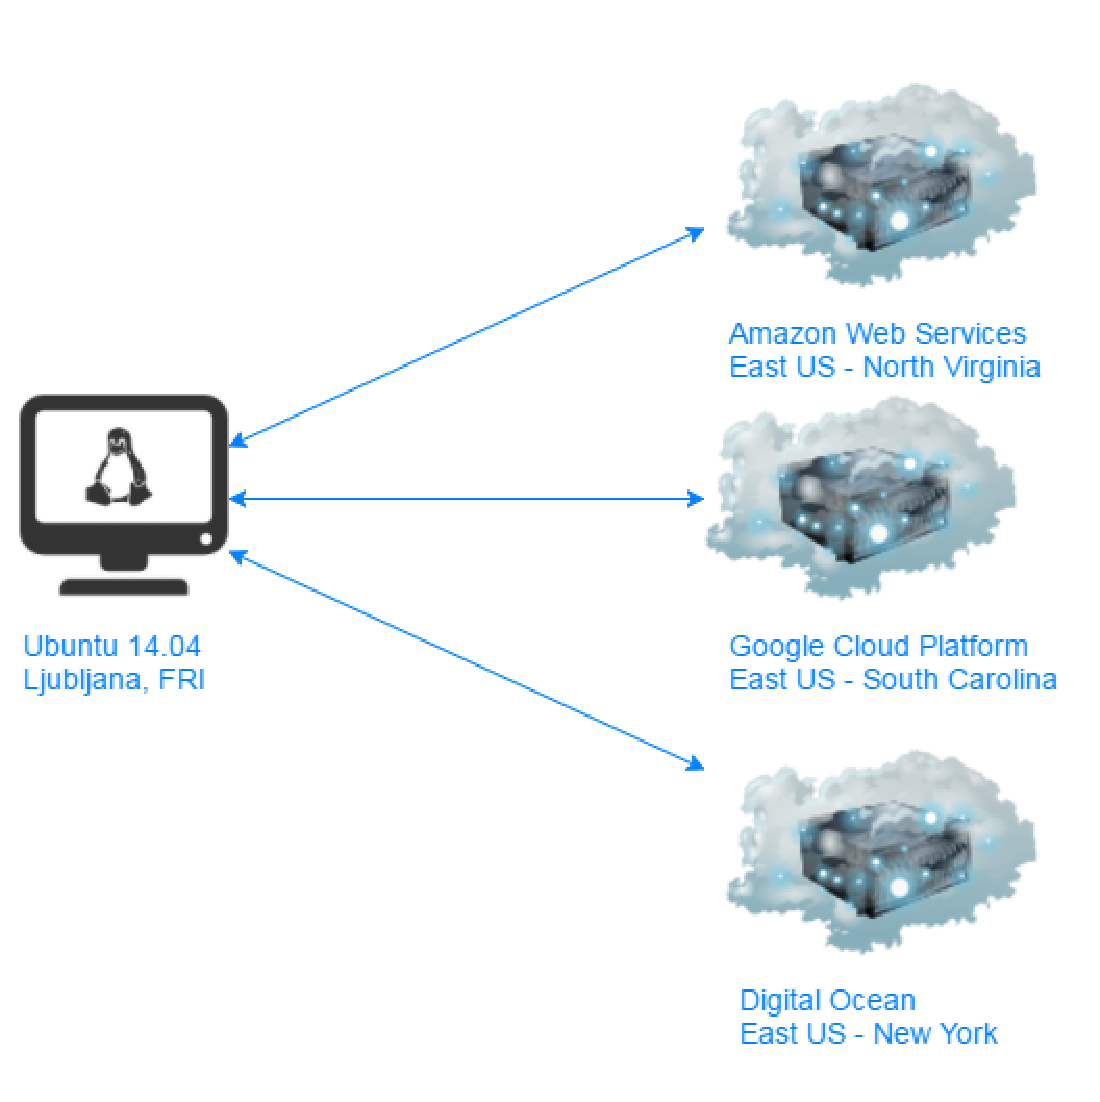
\includegraphics[width=0.8\textwidth]{1_cloudScheme}
  \caption{Shema testnega sistema.}
  \label{1_cloudSch}
\end{figure}

\section{Izbrane metrike}
V pri"cujo"cem poglavju so opisane izbrane metrike za merjenje zmogljivosti obla"cnega sistema.

\subsection{Prepustnost omre"zja}
Prepustnost omre"zja je eden klju"cnih dejavnikov dana"snjega komunikacijskega sveta. Vse ve"c podatkov se prena"sa preko omre"zja. Potreba po pomnilnih prenosnih medijih, s katerimi bi prena"sali podatke, prakti"cno izginja. Tako kot v vsakdanjem "zivljenju, je tudi pri obla"cnih storitvah seveda prenos podatkov preko omre"zja skorajda edina mo"znost. Posledi"cno gre za zelo zanimivo metriko s stali"s"ca kon"cnih uporabnikov. Vsakogar zanima kako hitro bo lahko prenesel svojega podatke iz to"cke A do to"cke B v omre"zju.

\subsection{Hitrost procesiranja}
Tudi hitrost procesiranja ima velik pomen, saj danes na ra"cunalniku ne te"ce ve"c samo en proces oziroma aplikacija, ampak je teh aplikacij mnogo in se morajo zato boriti za procesorski "cas. Kon"cni uporabnik "zeli vedno imeti ob"cutek teko"cega delovanja sistema, kljub temu da hkrati uporablja ve"c aplikacij ali servisov. Zmogljivost procesne enote (CPE) je tako zelo pomembna, saj omogo"ca hitro procesiranje zahtev in tako mo"znost delovanja tudi ostalih aplikacij na sistemu. "Ce bi recimo ena operacija na procesorju porabila preve"c "casa, bi posledi"cno ostali procesi obstali in bi uporabnik dobil ob"cutek, da sistem ne deluje najbolje.

\subsection{Zmogljivost datote"cnega sistema}
Zmogljivost datote"cnega sistema je izrednega pomena pri prenosu podatkov, bodisi da gre za prenos preko omre"zja ali lokalni prenos med razli"cnimi shranjevalnimi mediji. To ne zajema zgolj ro"cnega kopiranja datotek, ampak tudi vse interne prenose podatkov, ki jih opravljajo aplikacije. Gre za enega izmed kriterijev, ki je tudi zelo zanimiv za kon"cnega uporabnika, saj predstavlja operacije s katerimi se uporabniki sre"cujejo dnevno.

\section{Opis bremena}
V pri"cujo"cem razdelku so na kratko opisana vsa bremena, ki smo jih uporabljali pri testiranju.

\subsection{Iperf}
Prepustnost omre"zja za promet po protokolarnem skladu TCP/IP lahko enostavno izmerimo z orodjem \textit{Iperf} \cite{1_iperf}. \textit{Iperf} deluje kot obi"cajna TCP storitev, in sicer na eni strani povezave je stre"znik, na drugi pa odjemalec. Odjemalec generira in po"silja zahteve, ki predstavljajo breme, na drugi strani pa je stre"znik v vlogi prejemnika zahtev. \textit{Iperf} izmeri koli"cino prenesenih podatkov in na podlagi znanega trajanja meritve izra"cuna hitrost prenosa podatkov. Rezultat torej predstavlja hitrost prenosa podatkov v bitih na sekundo (bps). Pri velikih hitrostih povezav in dalj"sih "casih potovanja paketov med stre"znikom in odjemalcem je zelo pomembna velikost okna v TCP/IP skladu (angl. \textit{TCP buffer size}). V lokalnem ethernet omre"zju so "casi potovanja paketov zelo kratki, zato obi"cajna velikost okna za TCP povsem zado"s"ca. Priporo"cena velikost okna je enaka produktu hitrosti povezave in "casa potovanja paketa (angl. \textit{round trip time}). Privzeta velikost je 32 KB. Na primer v lokalnem 100 Mb/s omre"zju z zakasnitvijo 1 ms zado"s"ca "ze okno veliko 16 KB. 

\subsection{CoreMark}
\textit{CoreMark} \cite{1_coremark} je preprosto testno orodje za testiranje centralno procesnih enot (CPE). Njegova uporaba je zelo raz"sirjena in ima mo"znost, da postane del standardne specifikacije, vsaj kar se ti"ce osnovnega testiranja hitrosti procesiranja. Je neodvisen od procesorske platforme in tako omogo"ca primerjavo razli"cnih platform med sabo. Rezultat testa predstavlja deseti"ska vrednost, ki je se"stevek rezultatov vseh internih testov, ki jih uporablja \textit{CoreMark}, kar omogo"ca hitro in u"cinkovito primerjavo rezultatov. Program je napisan v programskem jeziku C in breme gradi na implementacijah splo"sno znanih algoritmov: iskanje in urejanje povezanih seznamov (uporaba kazalcev v pomnilniku), osnovne matri"cne matemati"cne operacije, 'state machine' (za simulacijo razli"cnih protokolov) in CRC (angl. \textit{cyclic redundancy check}, ki se uporablja v mno"zici protokolov predvsem za odkrivanje in popravljanje napak v podatkih). S pomo"cjo omenjenih bremen nam test prika"ze zmogljivost procesorskega sistema iz perspektive zmogljivosti podatkovnih vodil v sistemu, hitrosti pomnilnika in obstoje"cega predpomnilnika ter hitrosti procesiranja ra"cunskih operacij.

\subsection{FIO}
\textit{Fio} (angl. \textit{Flexible IO}) predstavlja orodje, ki generira breme, nato pa s pomo"cjo tega bremena testira in analizira delovanje datote"cnega sistema \cite{1_fio}. Gre za lokalni transport podatkov in ne za transport podatkov preko omre"zja. \textit{Fio} sestavljata dva dela: prvi del je definiranje bremena, kjer uporabnik definira ali se bo testiralo branje ali pisanje, "stevilo poslov, velikost posameznega posla ter velikost posameznega bloka za vhodno/izhodno operacijo. Drugi del predstavlja testiranje. Po uspe"snem zaklju"cku testa uporabnik pridobi informacije o hitrosti branja in pisanja, minimalno, maksimalno in povpre"cno latenco pri branju ali pisanju posameznega bloka, "stevilo iops (angl. \textit{input/output operations per second}), itd. 

\section{Rezultati meritev}
V tem razdelku so opisani postopki izvajanja testov in analize rezultatov, ki so bili pridobljeni po izvedenih testih. Vse teste smo izvajali na operacijskem sistemu Ubuntu 14.04. Teste smo pognali sredi tedna, torej v sredo, izvedli pa smo jih 24-krat - na vsako polno uro. Pri vsakem tipu meritev je tako podana tudi tabela z osnovnimi statisti"cnimi postavkami - minimum, maksimum, povpre"cje ter standardna deviacija meritev. Pri orodju \textit{Fio} je testov razmeroma veliko - skupno ve"c kot 700 - zatorej smo se odlo"cili, da v statisti"cni analizi predstavimo le dve, za uporabnika morda najpomembnej"si metriki - to sta bralna in pisalna hitrost.

\subsection{Testiranje prepustnosti omre"zja}
Za testiranje prepustnosti omre"zja smo uporabili orodje \textit{Iperf}. Breme pri testiranju prepustnosti omre"zja predstavljajo zahteve za prenos datotek. Datoteke se po"siljajo od oblaka proti uporabniku in od uporabnika proti oblaku. Na podlagi prenesene koli"cine datotek (v MB) in prete"cenega "casa izra"cunamo povpre"cno hitrost prenosa po omre"zju.
Virtualne ra"cunalnike smo locirali na vzhodni obali ZDA (East US). Pri izvajanju testa smo merili internetno povezavo med entitetami v omre"zju. Ena izmed entitet je slu"zila kot obla"cna storitev, druga pa kot uporabnik, ki do storitve dostopa. Test smo izvedli obojesmerno (torej od oblaka proti uporabniku in obratno). \textit{Iperf} test se je v vsakem primeru izvajal 60 sekund.

Hitrosti po"siljanja podatkov proti oblaku posameznega ponudnika obla"cne storitve so vidne na sliki \ref{1_upIperf}. Ob"cutno najmanj"so zmogljivost prenosa smo odkrili pri ponudniku Amazon (AWS), kjer je bila povpre"cna hitrost prenosa pod 200 Mbit/s. Najve"cjo povpre"cno hitrost prenosa smo izmerili pri ponudniku Google (GCP), ki je le za odtenek premagal re"sitev Digital Ocean (DO). Obe vrednosti presegata hitrost 900 MBit/s in GCP se zelo pribli"za meji 1 Gbit/s. Pri GCP, kot tudi pri DO se je tako izkazalo, da imata ve"c kot 4x ve"cjo povpre"cno hitrost nalaganja datotek v oblak, v primerjavi s ponudnikom AWS.

\begin{figure}[H]
  \centering
    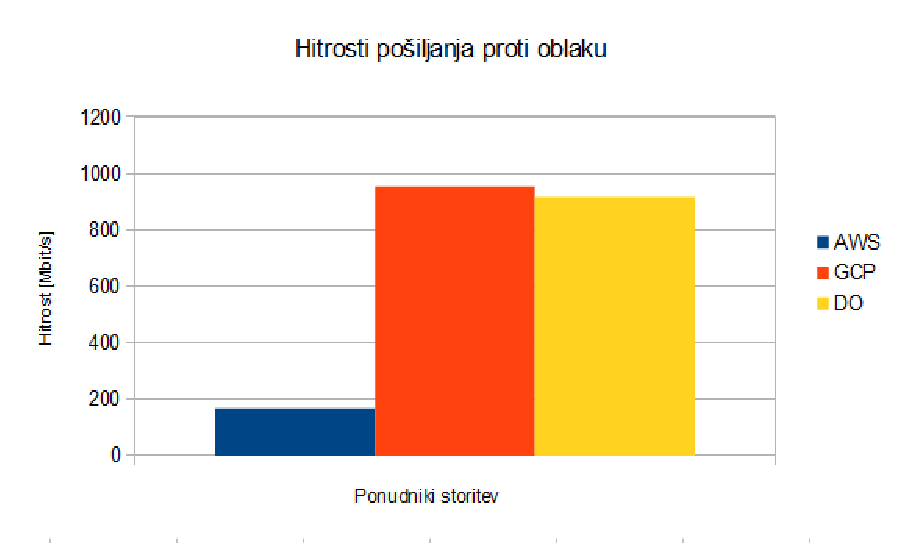
\includegraphics[width=0.8\textwidth]{1_uploadIperf}
  \caption{Povpre"cna hitrost pri prenosu podatkov proti oblaku (angl. \textit{upload speed}).}
  \label{1_upIperf}
\end{figure}

Na sliki \ref{1_table_upIperf} so razvidni osnovni statisti"cni podatki za meritve \textit{Iperf - upload}. Do najve"cjih odstopanj med minimalno in maksimalno vrednostjo je pri"slo pri ponudniku AWS, "ceprav ima dale"c najslab"si povpre"cni rezultat. Najbolj stabilno in povpre"cno tudi najbolj"se se je odrezal GCP.

\begin{figure}[H]
  \centering
    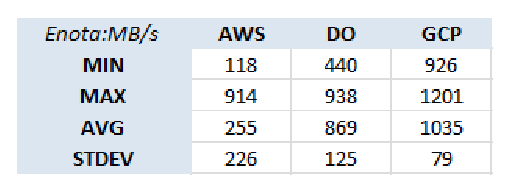
\includegraphics[width=0.8\textwidth]{1_table_iperf_ul}
  \caption{Statisti"cna analiza rezultatov \textit{Iperf - upload}.}
  \label{1_table_upIperf}
\end{figure}

Hitrosti po"siljanja podatkov proti uporabniku so vidne na sliki \ref{1_downIperf}. Zgodba je skoraj da identi"cna, kot pri hitrostih prenosa v obratni smeri. Ob"cutno najhitrej"sa sta zopet GCP in DO, dale"c zadaj pa je ponovno AWS. Pri primerjavi hitrosti se je izkazalo, da je razmerje zmogljivosti prakti"cno enako, kot v prej"snjem primeru.

\begin{figure}[H]
  \centering
    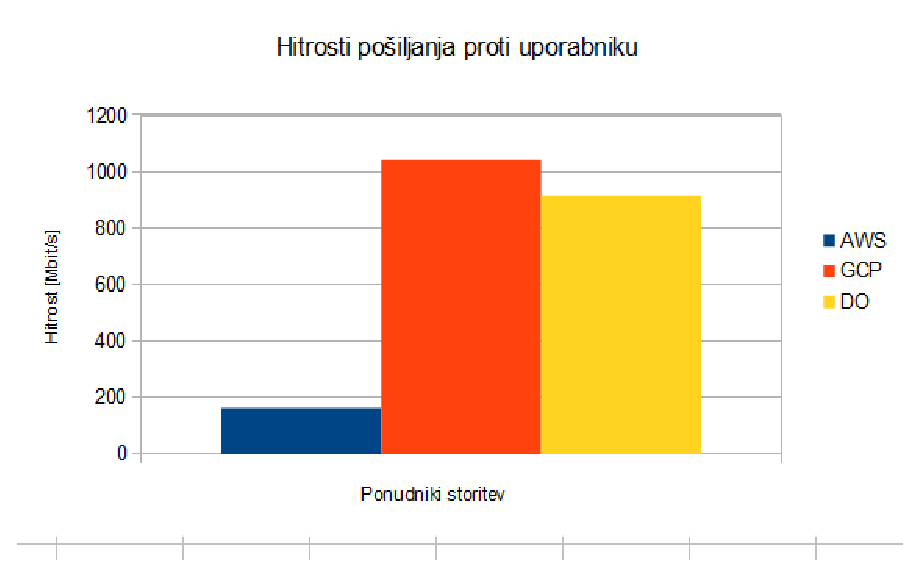
\includegraphics[width=0.8\textwidth]{1_downloadIperf}
  \caption{Povpre"cna hitrost pri prenosu podatkov proti uporabniku (angl. \textit{download speed}).}
  \label{1_downIperf}
\end{figure}

Tudi statisti"cna analiza \textit{Iperf - download} testa, vidna na sliki \ref{1_table_downIperf}, prikazuje podobne rezultate. Do najve"cje standardne deviacije rezultatov je pri"slo pri ponudniku AWS. DO in GCP pa sta pokazala precej bolj"se in bolj stabilne rezultate.

\begin{figure}[H]
  \centering
    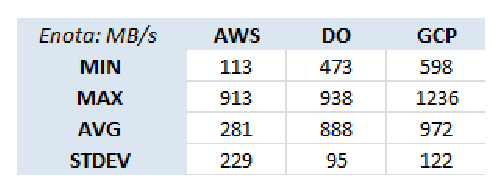
\includegraphics[width=0.8\textwidth]{1_table_iperf_dl}
  \caption{Statisti"cna analiza rezultatov \textit{Iperf - download}.}
  \label{1_table_downIperf}
\end{figure}


\subsection{Testiranje hitrosti procesiranja}
Procesorsko mo"c smo merili z orodjem \textit{CoreMark}. Breme pri testiranju hitrosti procesiranja predstavljajo splo"sni algoritmi kot so npr. iskanje in urejanje po seznamih, osnovne matri"cne operacije ter izvajanje CRC. Ker pri nobenem ponudniku nismo imeli izbire, kateri procesor bomo imeli na razpolago, je ta test zanimiv predvsem iz stali"s"ca procesorsko bolj zahtevnih aplikacij oziroma uporabnikov. Kot je razvidno iz slike \ref{1_core}, je najbolj zmogljiv procesor na voljo pri ponudniku Google Cloud, pri katerem rezultat testa presega 14.000 to"ck. Tesno mu sledi Amazon Web Services, z le nekaj manj kot 14.000 to"ckami, medtem ko je procesor pri DigitalOcean-u nekoliko manj zmogljiv, in se s skoraj 4000 tockami manj uvr"s"ca v \textit{CoreMark} rang 10.000 to"ck. Pri vseh ponudnikih smo pazili, da smo izbrali tak"sne storitve, ki niso trenutno deljene med druge uporabnike (torej imamo pri testiranju na voljo vso procesorsko mo"c; to nam zagotavlja ponudnik). Obstajajo namre"c tudi re"sitve, kjer je procesorska mo"c deljena med mnoge uporabnike hkrati, imamo pa le zagotovilo, da imamo v nekem trenutku vedno na razpolago nek odstotek skupne procesorske mo"ci (npr. 10\%).

\begin{figure}[H]
  \centering
    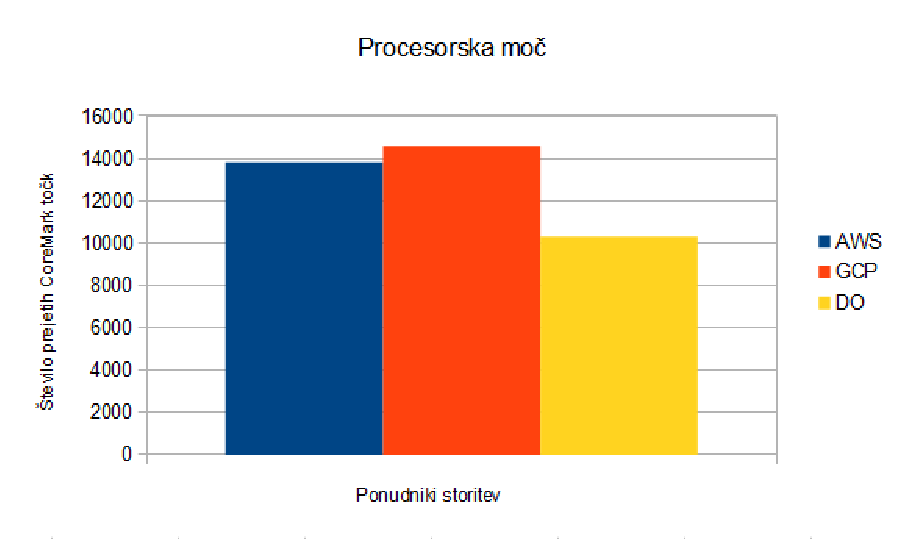
\includegraphics[width=0.8\textwidth]{1_coremark}
  \caption{"Stevilo prejetih \textit{CoreMark} to"ck.}
  \label{1_core}
\end{figure}

Statisti"cni podatki, ki izhajajo iz \textit{CoreMark} testa zmogljivosti procesorskega sistema so vidni na sliki \ref{1_table_core}. Povpre"cna rezultata AWS in GCP sta podobna in tudi standardna deviacija je skoraj enaka. Pri testu DO je pri"slo do anomalije in sicer se je pri eni izmed ponovitev testa zgodila napaka, ki je privedla do rezultata 0. Ta rezultat je delno pokvaril vrednosti ostalih statisti"cnih kazalcev.

\begin{figure}[H]
  \centering
    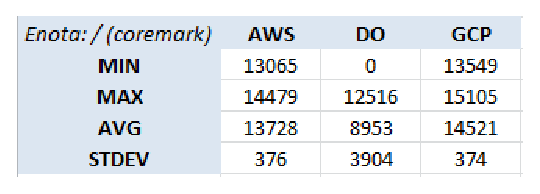
\includegraphics[width=0.8\textwidth]{1_table_coremark}
  \caption{Statisti"cna analiza rezultatov \textit{CoreMark}.}
  \label{1_table_core}
\end{figure}


\subsection{Testiranje zmogljivosti datote"cnega sistema}
Pri testiranju datote"cnega sistema smo se poslu"zili orodja \textit{Fio}. Preden smo teste izvedli, se je bilo potrebno odlo"citi za posamezne parametre (definiranje bremena). Breme je definirano v \textit{.job} datoteki, kjer se definirajo parametri kot so velikost bremena samega, velikost posameznega bloka, IO tip (ali gre za bralno ali pisalno operacijo), "stevilo datotek ("cez koliko datotek je breme razporejeno), itd. Velikost bloka smo nastavili na 512KB. Pri testiranju smo zahtevali izvedbo enega posla, ki smo mu nastavili razli"cne velikosti. Kot opombo bi vnaprej omenili, da platformi Amazon Web Services (AWS) in Google Cloud (GCP) uporabljata standardne trde diske, pri platformi Digital Ocean (DO) pa smo imeli na voljo SSD diske.

Na slikah \ref{1_avgR} in \ref{1_avgW} so prikazani rezultati za povpre"cno hitrost pri bralnih ter pisalnih operacijah. Platforma Digital Ocean ima pri"cakovano najve"cjo hitrost branja in pisanja, saj te"ce na SSD diskih. Bolj zanimiva je primerjava platform AWS in GCP. Povpre"cni hitrosti branja sta pribli"zno enaki. Razlika se pojavi pri hitrosti pisanja, kjer pa ima GCP ve"c kot 2x ve"cjo hitrost kot AWS. DO kot "ze re"ceno tukaj ni primerljiv, saj re"sitev te"ce na novej"si pomnilni"ski tehnologiji, katere bralno pisalne hitrosti dale"c presegajo klasi"cni diskovni sistem.

\begin{figure}[H]
  \centering
    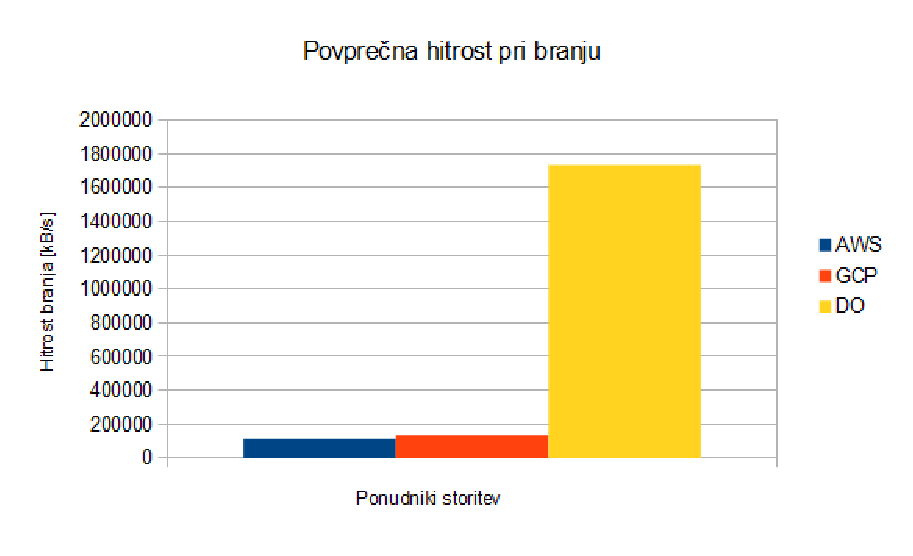
\includegraphics[width=0.8\textwidth]{1_povpBranje}
  \caption{Povpre"cna hitrost pri branju.}
  \label{1_avgR}
\end{figure}

\begin{figure}[H]
  \centering
    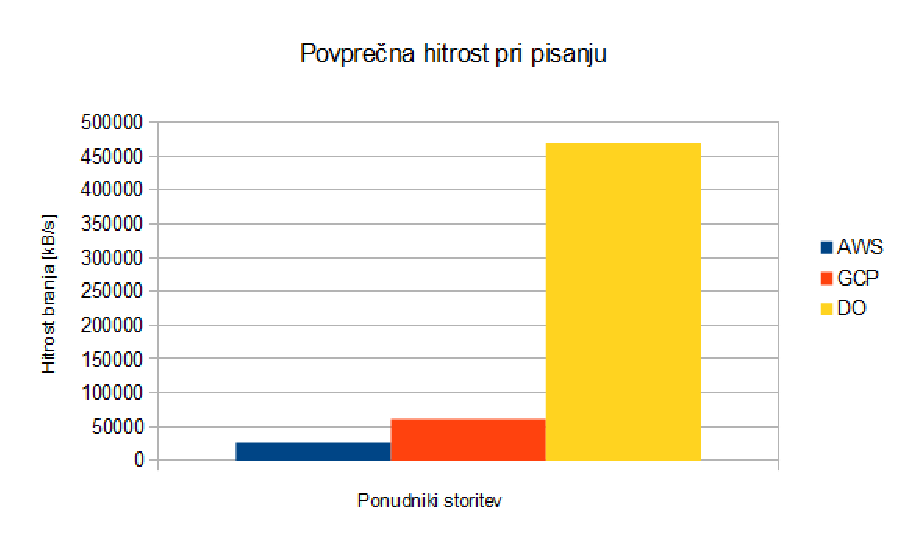
\includegraphics[width=0.8\textwidth]{1_povpPisanje}
  \caption{Povpre"cna hitrost pri pisanju.}
  \label{1_avgW}
\end{figure}

Glede na to, da platforma DigitalOcean uporablja SSD diske in ima s tem veliko prednost pred ostalima dneva ponudnikoma, je na sliki \ref{1_AvsG} prikazana "se primerjava bralne in pisalne hitrosti samo za platformi AWS in GCP. Kot smo "ze omenili v prej"snjem odstavku sta bralni hitrosti pribli"zno enaki, pisalna hitrost pa je pri GCP ve"c kot 2x ve"cja od AWS.

\begin{figure}[H]
  \centering
    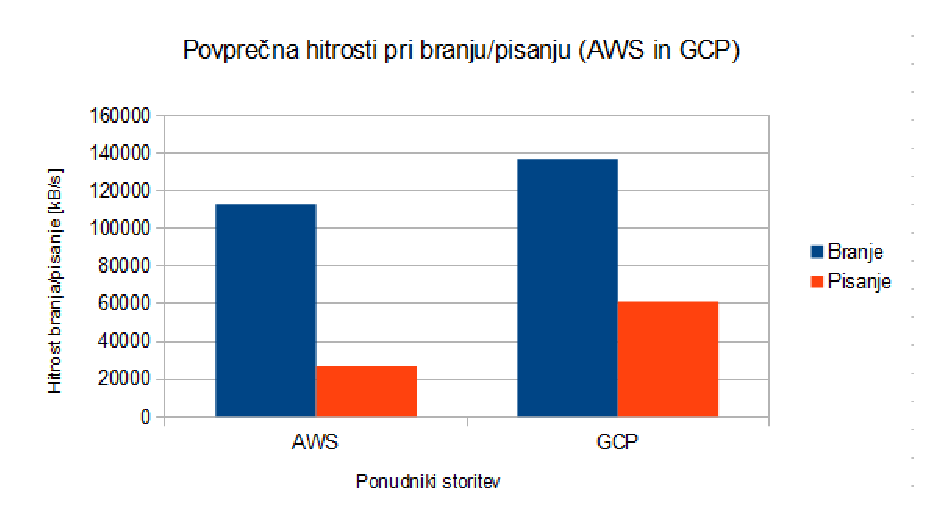
\includegraphics[width=0.8\textwidth]{1_AWSvsGCP}
  \caption{Povpre"cna hitrost pri branju in pisanju za platformi AWS in GCP.}
  \label{1_AvsG}
\end{figure}

Na slikah \ref{1_table_avgR} in \ref{1_table_avgW} je prikazana statisti"cna analiza rezultatov \textit{Fio - branje} in \textit{Fio - pisanje}. Rezultati AWS in GCP so ob"cutno slab"si, zaradi "ze prej omenjenih razlogov. Presenetljivo pa je velika standardna deviacija pri rezultatih DO, kljub temu da je povpre"cni rezultat ob"cutno bolj"si kot pri konkurentih, so odstopanja velika. Vzroke gre iskati v SSD tehnologiji sami, ki res da ponuja vi"sje maksimalne hitrosti, a je tudi sama hitrost bolj nepredvidljiva in odvisna od ve"c dejavnikov.

\begin{figure}[H]
  \centering
    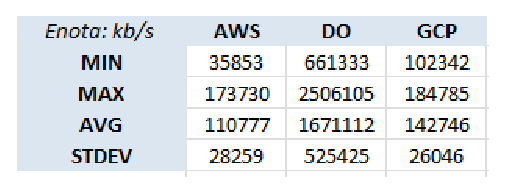
\includegraphics[width=0.8\textwidth]{1_table_fio_read}
  \caption{Statisti"cna analiza rezultatov \textit{Fio - branje}.}
  \label{1_table_avgR}
\end{figure}

\begin{figure}[H]
  \centering
    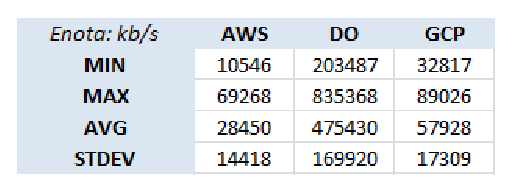
\includegraphics[width=0.8\textwidth]{1_table_fio_write}
  \caption{Statisti"cna analiza rezultatov \textit{Fio - pisanje}.}
  \label{1_table_avgW}
\end{figure}

Naslednja metrika, ki smo si jo ogledali pri testiranju podatkovnega sistema je latenca ene vhodno/izhodne operacije za posamezen blok podatkov. Rezultati so vidni na slikah \ref{1_latencyR} (branje) in \ref{1_latencyW} (pisanje). Platforma DO ima najmanj"se latence, zaradi "ze prej omenjenega razloga (SSD disk), zanimivej"si pa so rezultati latenc branja in pisanja pri platformah AWS in GCP. GCP ima sicer minimalno latenco branja precej manj"so, kot je minimalna latenca pri AWS, in tudi povpre"cna vrednost je nekoliko ni"zja. Druga"ce so pa rezultati latenc pri branju dokaj primerljivi. Ve"cja razlika se pojavi pri latenci pisanja, kjer so razlike precej ve"cje. GCP ima precej manj"so povpre"cno latenco branja, kar je seveda ugodneje. To je bilo pravzaprav za pri"cakovati, saj smo opazili tudi precej ve"cji razkorak v samih hitrostih pisanja pri teh dveh platformah.

\begin{figure}[H]
  \centering
    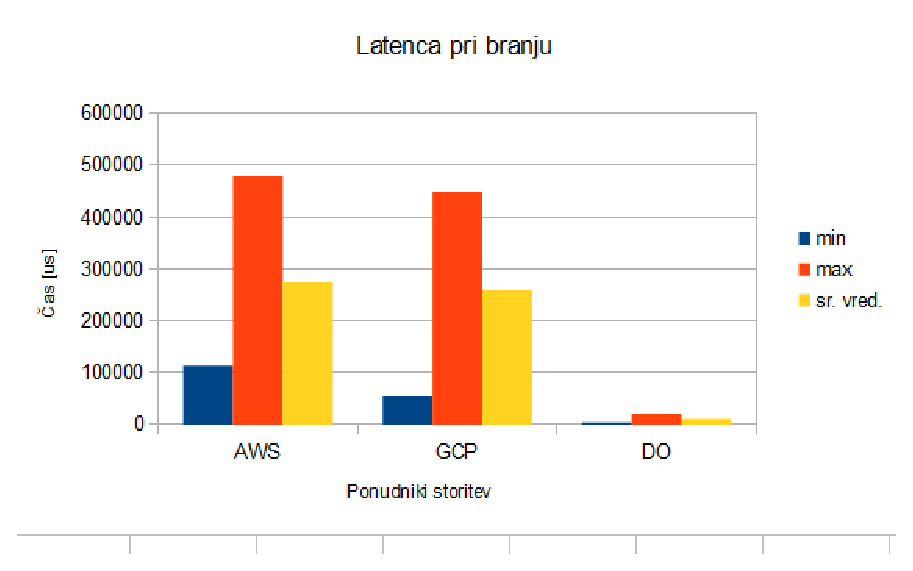
\includegraphics[width=0.8\textwidth]{1_readLatency}
  \caption{Minimalna, maksimalna in povpre"cna latenca pri branju enega bloka.}
  \label{1_latencyR}
\end{figure}

\begin{figure}[H]
  \centering
    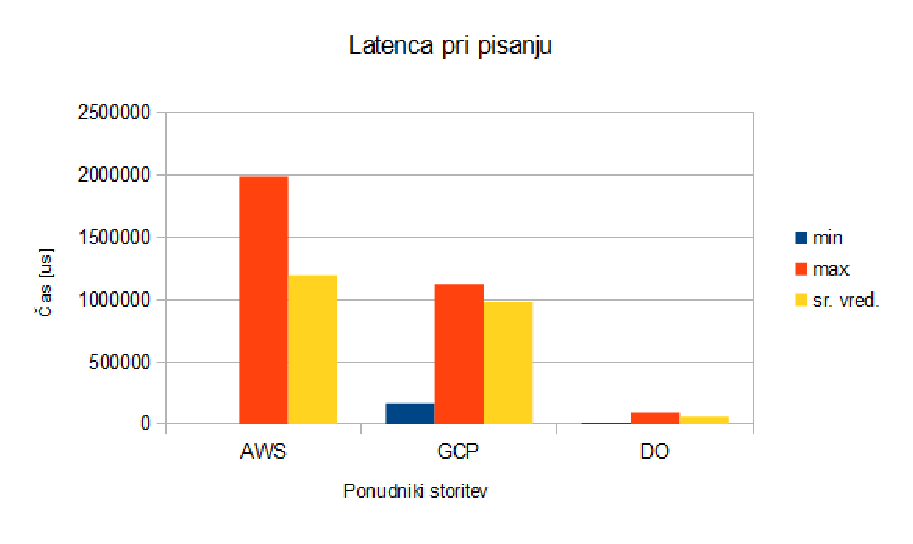
\includegraphics[width=0.8\textwidth]{1_writeLatency}
  \caption{Minimalna, maksimalna in povpre"cna latenca pri pisanju enega bloka.}
  \label{1_latencyW}
\end{figure}

Za zadnjo metriko smo si izbrali "stevilo vhodno/izhodnih operacij na sekundo. Rezultati so vidni na slikah \ref{1_iopsR} in \ref{1_iopsW}. Iz prej"snjih dveh analiz (hitrost in latenca) je mo"c pri"cakovati podobno razmerje mo"ci tudi pri "stevilu vhodno/izhodnih operacij. Platforma DO ima pri"cakovano najve"cje "stevilo operacij, tako pri branju kot pri pisanju. Pri platformah AWS in GCP pa je ponovno opazna podobnost pri bralnih operacijah, pri "stevilu pisalnih operacij pa je zopet ve"cja razlika, in sicer GCP je v primerjavi z AWS pri pisalnih operacijah ponovno ve"c kot 4x zmogljivej"si .

\begin{figure}[H]
  \centering
    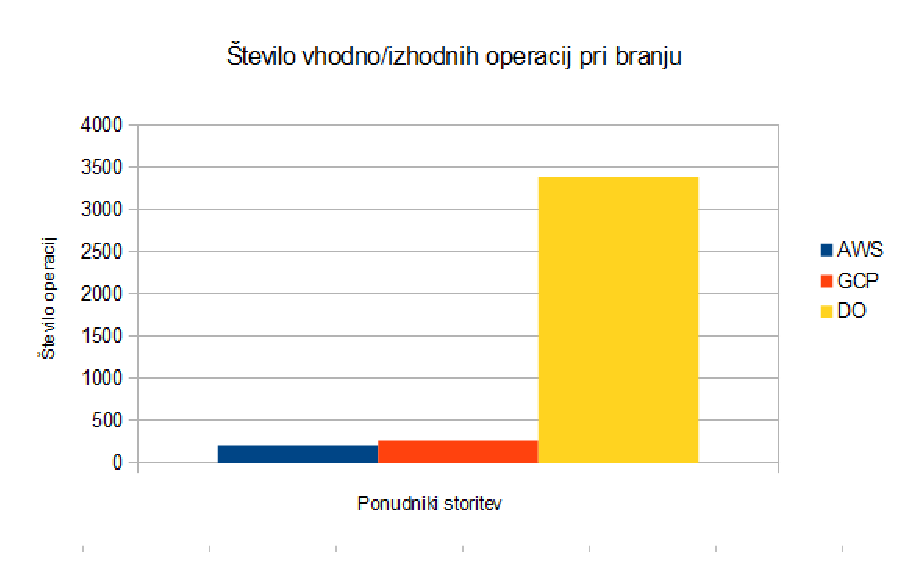
\includegraphics[width=0.8\textwidth]{1_iopsBranje}
  \caption{"Stevilo vhodno/izhodnih operacij pri branju.}
  \label{1_iopsR}
\end{figure}

\begin{figure}[H]
  \centering
    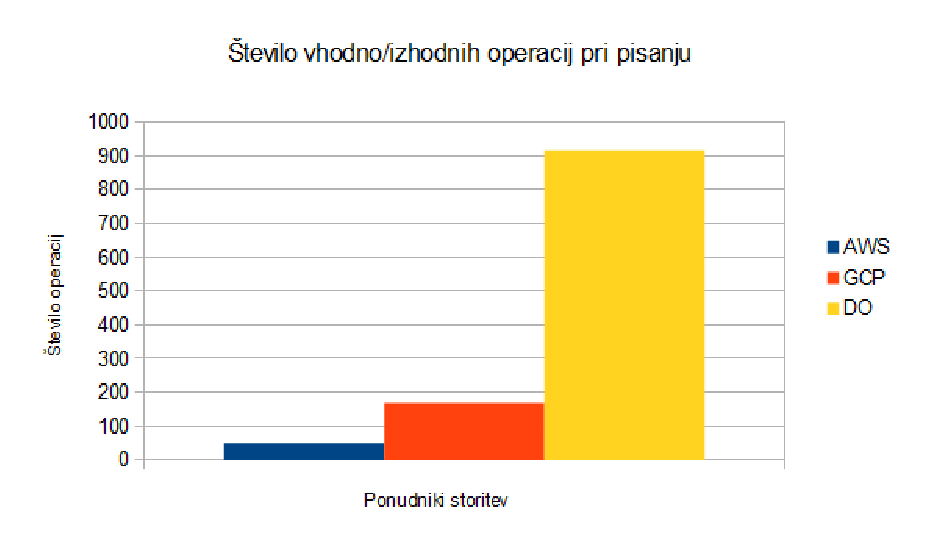
\includegraphics[width=0.8\textwidth]{1_iopsPisanje}
  \caption{"Stevilo vhodno/izhodnih operacij pri pisanju.}
  \label{1_iopsW}
\end{figure}

\section{Komentarji rezultatov}
Katerega ponudnika torej izbrati? Kot lahko razberemo iz rezultatov, ima vsak ponudnik svoje prednosti in slabosti.
Za uporabnike, ki potrebujejo veliko hitrih I/O operacij, hkrati pa niso preve"c zahtevni glede zmogljivost procesorja, je DigitalOcean zagotovo prva izbira, saj novej"sa pomnilni"ska tehnologija omogo"ca neprimerljivo vi"sje hitrosti bralno pisalnih operacij. Google Cloud Platform ponuja izjemno hitrost prenosa po njihovih opti"cnih povezavah, hkrati pa ima tudi rahlo bolj"so procesorsko mo"c ter hitrost I/O operacij od njihovega rivala Amazon Web Services.
Splo"sno gledano, se je od vseh najslab"se odrezal prav AWS, saj v nobeni izmed kategorij ni bil najbolj"si.
Kot "ze omenjeno, pa je izbira v veliki meri odvisna od samega uporabnika ter namena 
uporabe storitve, deloma pa tudi od drugih zunanjih dejavnikov, kot so npr. lokacija, cena, osebne preference in ostale omejitve.